%% Settings for single-side (simplex) printing
% Margins: left 40mm, right 25mm, top and bottom 25mm
% (but beware, LaTeX adds 1in implicitly)
\documentclass[12pt,a4paper]{report}
\setlength\textwidth{160mm}

\usepackage[utf8]{inputenc}
\usepackage{graphicx}
\usepackage{fancyhdr}
\usepackage{lmodern}
\usepackage{lastpage}
\usepackage{subfig}
\usepackage{hyperref}

\graphicspath{{../graphs/}}

\pagestyle{fancy}
\fancyhf{}
\rhead{Petr Houška `houskape@gmail.com`}
\lhead{HW3: Matrix transposition}
\rfoot{Page \thepage / \pageref{LastPage}}


\begin{document}
	
	\begin{figure}[h]	
		\centering	
		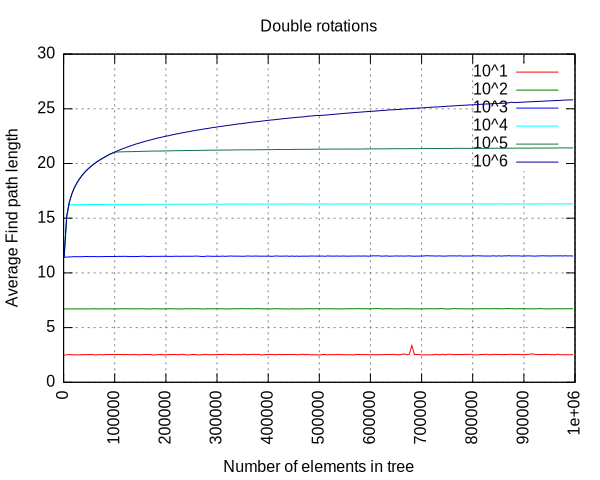
\includegraphics[scale=0.6]{graph_1}		
	\end{figure}
\
	Na prvním grafu vidíme porovnání průměrného času na prohození dvou prvků pro naivní algoritmus a rekurzivní cache oblivious algoritmus, který se zastaví na podmatici velikosti 8x8 a dál pokračuje naivně. 
	
	Pro cache oblivious algoritmus jsou zřejmé dva segmenty. Do cirka $1000^2$ prvků a od cirka $1000^2$ prvků. Skok mezi těmito dvěma segmenty ovšem není nikterak výrazný, z $1.5 * 10^{-6}$ na $4.0 * 10^{-6}$.
	
	U naivního algoritmu jsou segmenty pozorovatelné 3. Od začátku do $1000^2$ prvků, kde se průměrný čas pohybuje okolo $1.5 * 10^{-6}$, tedy stejně jako u cache oblivious algoritmu, následně do 	$15000^2$ prvků okolo $1-2 * 10^{-5}$ a nakonec je pozorovatelný skok k $5*10^{-5}$.

	\begin{figure}[h]	
	\centering	
	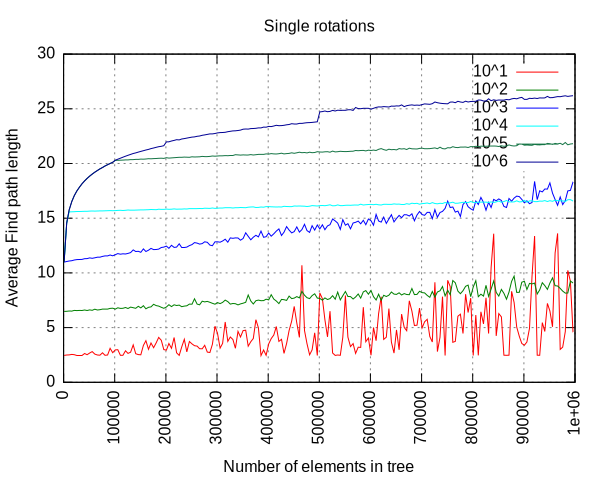
\includegraphics[scale=0.6]{graph_2}		
	\end{figure}

	Na grafu ze simulátoru jsou 

	\begin{figure}[h]	
    \centering
		\subfloat{{\includegraphics[scale=0.4]{graph_2_adv}}}%
		\qquad
		\subfloat{{\includegraphics[scale=0.4]{graph_2_naive}}}%
    \end{figure}




\end{document}